\chapter{Time Complexity}
\section{Measuring Complexity}
\begin{yellowBox}
	\begin{defn}[\TIME]
		For a function $t:\NN\to \NN$ we define
		\[
		\TIME(t(n)) = \cbk{\Ll\mid\text{ $\exists\Mm$ that decides $\Ll$ for $|w|=n$, halts after $O(t(n))$ steps}}
		\]
	\end{defn}
\end{yellowBox}
\begin{example}
	For $\Ll_{eq} = \{0^n1^n\}$ we saw $\Ll_{eq}\in \TIME(n^2)$. In fact - $\Ll_{eq} \in \TIME(n\log n)$\footnote{In every iteration - delete half of the $0$s and $1$s that survived until the current stage}.\\
	A TM with two strips can decide $\Ll_{eq}$ in $O(n)$ steps: Copy the $0$ prefix to the second strip and compare. Even though - $\Ll_{eq}\notin \TIME(n)$.\footnote{In fact - $\Ll\in \TIME(g(n))$ for $g\in o(n\log n)$ then $\Ll\in \Reg$. }
\end{example}
\begin{blueBox}
	\begin{thm}
		Let $t(n)$ be a function that satisfies $t(n) \geq n$\footnote{If $t(n)\leq n$ then we don't have time to read the input - so this is a reasonable assumption.}, then for any multi-strip TM that runs in $t(n)$ time, there is an equivalent single strip TM that runs in $t^2(n)$ time.
	\end{thm}
\end{blueBox}
\begin{proof}
	No Proof.
\end{proof}
\begin{blueBox}
	\begin{thm}
		If $t(n) \geq n$, and a nondeterministic TM that runs within $t(n)$ time, there is a deterministic single strip TM that runs within $2^{O(t(n))}$ time.
	\end{thm}
\end{blueBox}
\begin{yellowBox}
	\begin{defn}[Nondeterministic Complexity classes]
		Define:
		\begin{itemize}
			\item $\NTIME(t(n)) = \cbk{\Ll\mid\small\text{ $\exists\Mm$ nondeterministic decider that for $|w| = n|$ halts after $O(n)$ steps}}$
			\item $\PTIME = \displaystyle\bigcup_{k\geq 0}\TIME(n^k)$, with the petname $\P$.
			\item $\NPTIME = \displaystyle\bigcup_{k\geq 0}\NTIME(n^k)$, with the petname $\NP$.
			\item $\EXPTIME = \displaystyle\bigcup_{k\geq 0}\NTIME(2^{n^k})$
		\end{itemize}
	\end{defn}
\end{yellowBox}
\begin{blueBox}
	\begin{thm}
		$\P\subseteq\NP\subseteq\EXPTIME$
	\end{thm}
\end{blueBox}
\begin{proof}
	Any deterministic TM is a nondeterministic TM (first containment) and any nondeterministic TM can be simulated by a deterministic TM in exponential time (second containment).
\end{proof}
\section{The classes $\P,\NP$}
Consider two classical problems on graphs: Euler paths and Hamiltonian paths. Let $G = (V,E)$ (simple undirected graph). Let $\Gg_E, \Gg_H$ be the languages of graphs with Euler and Hamilton paths (respectively), then $\Gg_E\in \P$ (even $\NTIME(O(n))$). But we don't know $\Gg_H\nim{?}\in \P$. With that said - we do know $\Gg_H\in \NP$ by guessing a permutation of the vertices.
\begin{example}
	Define the language $$D-ST-HAMPATH = \cbk{\tbk{G,s,t}\mid \text{$G$ is a Directed graph with hamiltonian path }s\to t}$$
	For example - this digraph has an Hamiltonian $s\to t$ path:
	\begin{figure}[H]
		\centering
		\begin{tikzpicture}[shorten >=1pt,node distance=3cm,on grid,auto]
			\node[state] (s)   {$s$};
			\node[state] (q_1) at (2,2) {};
			\node[state] (q_2) at (2,-2) {};
			\node[state] (q_3) at (4,1) {};
			\node[state] (q_4) at (4,-1) {};
			\node[state] (q_5) at (6,2) {};
			\node[state] (q_6) at (6,-2) {};
			\node[state] (t) at (8,0) {$t$};
			
			
			\path[-stealth, thick]
			(s) edge [blue] (q_2)
			(q_1) edge (s) edge (q_2) edge [blue] (q_5)
			(q_2) edge [blue] (q_4) edge (q_6)
			(q_3) edge [blue] (q_1)
			(q_4) edge [blue] (q_3) edge (q_6)
			(q_5) edge [blue] (q_6) edge (t)
			(q_6) edge [blue] (t)
			
			;
		\end{tikzpicture}
		\caption{Graph with Hampath $s\to t$}
	\end{figure}
	\begin{prop}
		$D-ST-HAMPATH \in \EXPTIME$
	\end{prop}
\begin{proof}
	Given $G,s,t$, let $\pi_1\ldots \pi_{n!}$ denote the permutations of $V(G)$:
	\begin{enumerate}
		\item While $i\leq n!$:
		\item Let $\pi_i = v_1^i\ldots v_n^i$
		\item If $v_1^i = s, v_n^i = t$ and $(v_j^i,v_{j+1}^i)\in E$ - accept. Otherwise $i+=1$.
	\end{enumerate}
This algorithm runs in exponential time.
\end{proof}
Note that it is easy to check a given permutation. The reason that the algorithm is exponential is due to the number of possibilities.\\
Also - $D-ST-HAMPATH \in \NP$. Consider the NTM that guesses a permutation $\pi$ and checks if it is an $s,t$ Hamiltonian path.\\
What about $D-ST-HAMPATH^c$ (all graphs with no Hamiltonian path). Once again it is in $\EXPTIME$, but\footnote{Probably} not in $\NP$!
\end{example}
\begin{example}
	$COMPOSITE = \{x\mid x = p\cdot q\}$, of course $COMPOSITE^c = PRIME$. By assumption - $x$ is given in binary, so $COMPOSITE\in \NP$: Deciding prime numbers for an unary represented number is indeed polynomial. Since the input's length (in binary) is logarithmic in the unary representation - the time complexity is actually exponential in the representation.
\end{example}
\begin{yellowBox}
	\begin{defn}[Verifier]
		For a language $\Ll$, a TM $\Vv$ is a \textbf{Verifier} of $\Ll$ if\[
		\Ll = \cbk{w\mid \text{$\Vv$ accepts $\tbk{c,v}$ for some $x\in \Sigma^*$}}
		\]
		The verifier's complexity is measured WRT $|w|$: That is, runs in $poly(|w|)$ time on $\tbk{w,c}$. This implies $|c| = poly(|w|)$.
	\end{defn}
\end{yellowBox}
\begin{blueBox}
	\begin{thm}[Alternative characterization]
		$\Ll\in \NP \iff$ there exists a polynomial verifier for $\Ll$.
	\end{thm}
\end{blueBox}
\begin{proof}
	Assume $\Vv$ is a verifier. Construct a polynomial NTM that guesses a word $c$ with $|c| = poly(|w|)$ (all words with $|c| \leq f(|w|)$ where $f$ is $\Vv$'s time complexity) and runs $\Vv$ over $\tbk{w,c}$. For the other side - let $\Ll\in \NP$, then define $\Vv$ to accept $\tbk{w,c}\iff c$ is an accepting run of $\Mm_\Ll$ on $w$. Correctness is obvious, and since $\Mm_\Ll$ is polynomial - $|c| = poly(|w|)$, hence $\Vv$ is polynomial.
\end{proof}
\begin{example}
	A verifier for $D-ST-HAMPATH$ is the machine $\Vv$ with 
	\[
	\Ll(\Vv) = \cbk{\tbk{G,s,t,\pi}\mid \pi\text{ is a Hamiltonian $s,t$ path}}
	\]
\end{example}
\begin{example}
	A verifier for $COMPOSITE$:\[
	\Ll(\Vv) = \cbk{\tbk{x,p,q}\mid x = p\cdot q\quad q,p\neq 1}
	\]
	Of course there are variations and different verifiers (e.g - only one devisor)
\end{example}
\section{$\NP$-Completeness}
We would like to show that some things are not in $\P$. However - this is hard: We would need to prove that no polynomial TM decides the language. For this - we define a class of languages that had they been in $\P$, then things break beyond repair. For that - we need some more definitions. Until now (in computability theore) we used reductions to show that some problems are not in $\Rcr$, or not in $\RE$. Now we care about time complexity - so we need to take care of that.
\begin{yellowBox}
	\begin{defn}[Polynomialy Computable]
		A function $f:\Sigma^*\to \Sigma^*$ is said to be \textbf{Polyninomialy computable} if there is a polynomial TM $\Mm$ that computes it.
	\end{defn}
\begin{defn}
	[Polynomialy Reducable
	] We say $A$ is \textbf{Polynomialy Reducable} to $B$ (denote $A\leq_p B$) if there is a poly-computable function $f:\Sigma^*\to \Sigma^*$ with
	\[
	w\in A \iff f(w)\in B
	\]
\end{defn}
\end{yellowBox}
\begin{blueBox}
	\begin{thm}[Reduction Theorem]
		If $A\leq_p B$ and $B\in \P$ then $A\in \P$.
	\end{thm}
\end{blueBox}
\begin{proof}
	Let $\Mm_b$ poly TM for $B$ with complexity function $t_B$, and $f$ a poly-reduction $A\leq_p B$. A TM that decides $A$: Given $w$ compute $f(w)$ in $t_f(|w|)$ time, and $f(|w|)\leq t_f(w)$. Now run $\Mm_B$ over $f(w)$ in no more than $t_b(t_f(w))$ which is polynomial in $|w|$.
\end{proof}
With these definitions, we can define "hard languages":
\begin{yellowBox}
	\begin{defn}
		[$\NP $ - hard]We say that $\Ll$ is \textbf{$\NP$-Hard} if 
		\[
		\forall \Ll'\in \NP \quad \Ll'\leq_p \Ll
		\]
	\end{defn}
	\begin{defn}
		[$\NP $ - complete]We say that $\Ll$ is \textbf{$\NP$-Complete} if $\Ll\in \NP$ and is $\NP$-hard.\\
	\end{defn}
\end{yellowBox}
\begin{blueBox}
	\begin{thm}
		Let $\Ll\in \NP$. Then
		$\Ll\in \NPcomplete \iff$ there exists an $\NP$ hard language $\Ll'$ such that $\Ll'\leq_p \Ll$.
	\end{thm}
\end{blueBox}
\begin{proof}
	$\Leftarrow$ By transitivity. $\Rightarrow$ By reflexivity.
\end{proof}
\begin{example}
	define $SAT = \cbk{\tbk{\Theta}\mid \Theta\text{ is satisfyable}}\in \NP$ (by guessing an assignment). This language is $\NP$ complete - we will show this later.
\end{example}
\begin{yellowBox}
\begin{defn}
	[Conjunctive Normal Form] 
	A \textbf{literal} is a Boolean variable or a negated Boolean variable, as in $x$ or $\neg x$.
	A \textbf{Clause} is several literals connected with $\vee$s, as in ($x_1 \vee x_2\vee x_3 \vee \neg x_4$). A boolean formula is in \textbf{conjunctive normal form}, called a \textbf{cnf-formula}, if it comprises several clauses connected with $\wedge$s
\end{defn}
\end{yellowBox}
\begin{example}
	Let $3SAT = \cbk{\tbk{\varphi}\mid \varphi\in 3CNF}$\footnote{That is, $\varphi$ is in CNF form with $3$ literals in any clause.}\\
	Define $CLIQUE = \cbk{\tbk{G,k}\mid \text{The graph $G$ has a clique of size }k}$. We show $3SAT\leq_p CLIQUE$. It is easy to show that $3SAT\leq_m CLIQUE$: Given $\Theta$, check if it is satisfyable (in exponential time). If so - write $\tbk{K_2,2}$ on the strip. If not - write $\tbk{K_2,3}$.\\ 
	We now show a polynomial reduction $3SAT\leq_p CLIQUE$. Let $f:\varphi\mapsto \tbk{G,k}$ be the following function: Given 
	\[
	\varphi = \bigwedge_{i\in [m]}(\ell_i^1\vee \ell_i^2 \vee \ell_i^3)
	\]
	Define $G$ with $V(G) = \cbk{\ell_i^1,\ell_i^2,\ell_i^3\mid i\in [m]}$ (all the literals in $\varphi$), let $k = m$ (the number of clauses) and \[E(G) = V\times V\setminus \left(\cbk{(u,v)\mid u,v\text{ are in the same clause}}\cup \cbk{(u,v)\mid u = \neg v}\right)\]
	This build is polynomial- since there are $3m$ vertices and $O(m^2)$ edges. As for correctness, assume $\varphi$ is satisfyable and let $\nu:X\to \{T,F\}$ a satisfying valuation of $\varphi$. Thus, in any clause $C_j$ of $\varphi$ there is at least one literal $\ell^{k_j}_j$ with $\nu(\ell^{k_j}_j) = T$ (since it is in CNF). 
	\begin{prop}
		The collection $\cbk{\ell_j^{k_j}}_{j\in[m]}$ defines a clique in $G(\varphi)$
	\end{prop}
\begin{proof}
	Indeed, $(\ell^{k_{j}}_{j}, \ell^{k_i}_i)\in E$ since they are not from the same clause and cannot be negations of one another - since they are valued the same under $\nu$.
\end{proof}
Conversely, assume $G$ has a clique of size $m$. By definition of $E$, the clique contains exactly one representative of any clause $C_j$, and the representatives are consistent under valuations. This defines a satisfying valuation $\nu$ of $\varphi$ (exercise).\\

An example of this build is shown:
\begin{figure}[H]
	\centering
	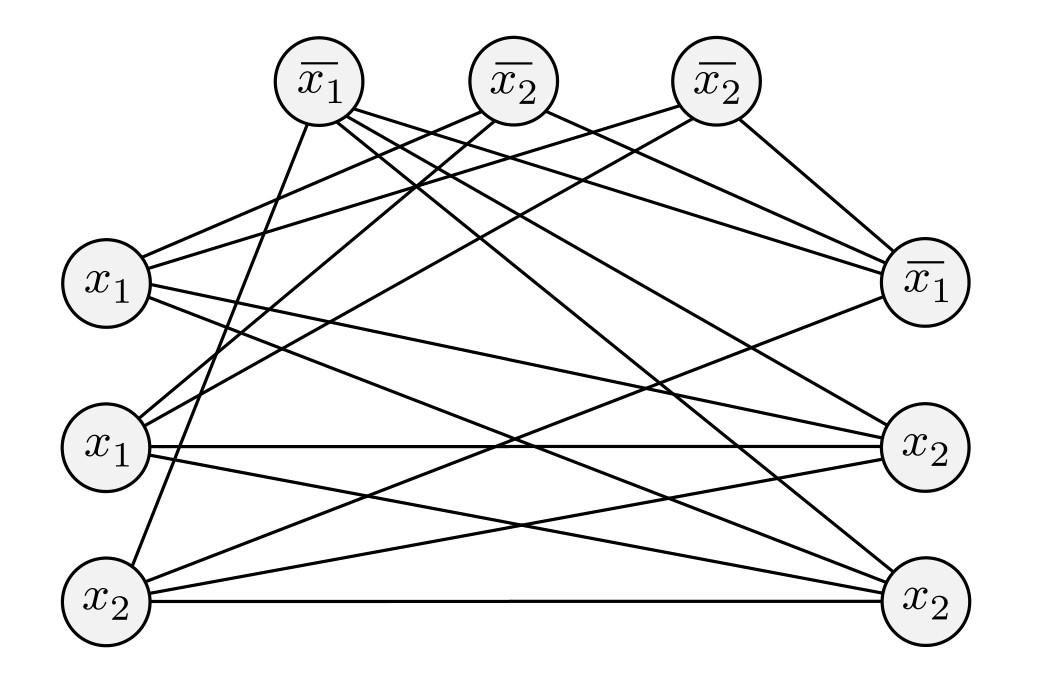
\includegraphics[scale=.4]{3satReduction.jpg}
	\caption{The build from $\phi = (x_1\lor x_1 \lor \neg x_2)\land (\neg x_1 \lor \neg x_2\ \lor \neg x_2) \land (\neg x_1 \lor x_2 \lor x_2) $}
\end{figure}
\end{example}
\begin{blueBox}
	\begin{thm}
		$\Ll$ is $\NP$-complete $\Rightarrow$ $(\Ll\in \P\Rightarrow \P = \NP)$.
	\end{thm}
\end{blueBox}
\begin{proof}
	Let $\Ll$ an $\NP$-complete language. Hence, for any $\Ll'\in \NP$ there is a poly-reduction $f_{\Ll'}$ from $\Ll'$ to $\Ll$. Therefore $\Ll\in \P$ implies that $\Ll'\in \P$. Since $\P\subset \NP$ we get $\P = \NP$.
\end{proof}
\begin{example}
	Consider the language of vertex cover $VC = \cbk{\tbk{G,k}\mid G\text{ has a vertex cover of size at most }k}$. We show that this language is $\NP$-Complete.
	\begin{prop}
		$VC\in \NP$
	\end{prop}
\begin{proof}
	Consider the verifier that gets as input $\tbk{G,k,S}$ with $S\subset V$ and checks that $|S| \leq k$, then traverses $E$ and checks for $e\in E$ if there is a vertex $v\in V$ that is incident with $e$. If this holds for all $e\in E$, accept, otherwise reject. This is clearly correct. As for time complexity - checking the size of $S$ is at most $|V(G)|$. For any edge we compare it against all $V$, so total runtime of $O(|E|\cdot |V|)$, hence the runtime is $poly(\abs{\tbk{G}})$
\end{proof}
\begin{prop}
	$VC$ is $\NP$-hard.
\end{prop}
\begin{proof}
	We show that $CLIQUE \leq_p VC$, which results in $VC$ being $\NP$ hard. Consider $f:\tbk{G,k}\mapsto \tbk{G^c,n-k}$ with $G^c$ the complement graph of $G$. \\
	Assume $G$ has a clique of size $k$ and $v_1\ldots v_k$ clique vertices in $G$. No two of them are connected in $G^c$, then taking $S = V\setminus\{v_i\}_{i\in [k]}$ is hence a vertex cover of $G^c$, of size $n-k$. Conversely - if $G^c$ has a vertex cover of size $n-k$, denoted $S = \{v_1 \ldots v_{n - k}\}$, then all $V\setminus S$ define a clique: If $x,y\in V\setminus S$, we want to show $\{x,y\}\in E$, that is $\{x,y\}\notin E(G^c) = E^c$. If $\{x,y\}\in E^c$, since $x,y\notin S$ - $S$ is not a vertex cover of $G^c$, contradiction. Hence $V\setminus S$ defines a $k$-clique.
	As for time complexity - inverting the edges takes $O(|E|)$ time, and $k\mapsto n-k$ takes $O(|V|)$.
\end{proof}
\end{example}
\begin{yellowBox}
	\begin{defn}
		Given $G$, a dominating set $D\subset V$ is a set such that for all $v\in V $, $d(v,S) \leq 1$.
	\end{defn}
\end{yellowBox}
\begin{example}
	Consider $\cbk{\tbk{G,k}\mid \text{ There exists a dominating set in $G$ of size $k$}}$. We show that $DS$ is $\NP$ complete.\\
	A polynomial verifies would receive $\tbk{G,k,C}$ and checks that $C$ is a dominating set: Over $v\in V$ check if $v\in C$, if not - check if for any edge incident with $v$ if the other incident is in $C$. If exists - accept. Otherwise, reject. This is $poly(|G|)$: Iterating over $V$ is $O(|V|)$, over the edges is $O(|C|) = O(|V|)$, then total runtime of $O(|V|^2|E|)$.\\
	We reduce $VC\leq_p DS$. Consider the mapping $f: \tbk{G,k}\mapsto \tbk{G',k'}$: for $e = (x,y)\in E(G)$, $f$ adds a new vertex $v_e$ and the edges $\{(x,v_e), (y,v_e)\}$ (we only enrich the graph). Then $f$ returns $G'$ with $V(G') = V\cup \{v_e\}_{e\in E(G)}$ and $E(G') = E\cup \{(x,v_e), (y,v_e)\}_{e\in E(G)}$. Finally - $f$ counts the isolated nodes in $G$ (say, $m$) and returns $\tbk{G', k + m}$.\\
	Time complexity is $O(|V| + 3|E|) = O(V + |E|) = poly(|G|)$.\\
	As for correctness - assume $G$ has a VC $C$ of size $k$, and denote $F$ the isolated nodes of $G$: $C\cup F$ is a DS in $G'$ of size at most $k + m$: For $v\in V(G')$, it is either in $F$ (isolated), or not. If it is not, and $v\in V(G)$ - $v$ is in an edge $\{v,u\}$ and since $C$ is a VC of $G$, and $v$ is of distance $1$ to $C$. If $v = v_e$ for some $e$, then $e = \{x,y\}$, WLOG $x\in C$ and thus the distance to $C$ is at most $1$.\\
	
	Conversely - assume $G'$ has a dominating set of size $k'$ - it must contain the isolated vertices of $G$, discard them and we are left with a set $S$ of size $k$. If some $v_e\in S$, substitute it for some $x\in e = \{x,y\}$. This is a dominating set (proof omitted for I am awfully tired).
 \end{example}
\section{Cook - Levin Theorem}
\begin{blueBox}
	\begin{thm}[Cook - Levin Theorem]
		$3SAT\in \NPcomplete$.
	\end{thm}
\end{blueBox}
\begin{proof}
	First, $3SAT\in \NP$ by the verifier $\Vv$ with the language $\tbk{\varphi, \nu}$ where $\nu$ is a satisfying valuation of $\varphi$. It is left to show $3SAT\in \NPhard$.\\
	Let $\Ll\in \NP$. Define $f:w\mapsto \varphi\in 3CNF$. $\varphi$ is satisfyable if there exists a valuation, and $w\in \Ll$ if there exists an accepting run over $\Mm$ NTM that decides $\Ll$ within $t(|w|) = t(n) poly(n)$ time.. So we need to match runs to valuations of $\varphi$. That is - there exists a sequence of configurations $C_0\ldots C_m$ which is an accepting run of $\Mm$ over $w$, and $m = t(n)$. We build a matrix that in its entries there are characters from $S = \{\#\}\cup Q \cup \Gamma$:
	\begin{figure}[H]
		\centering
%		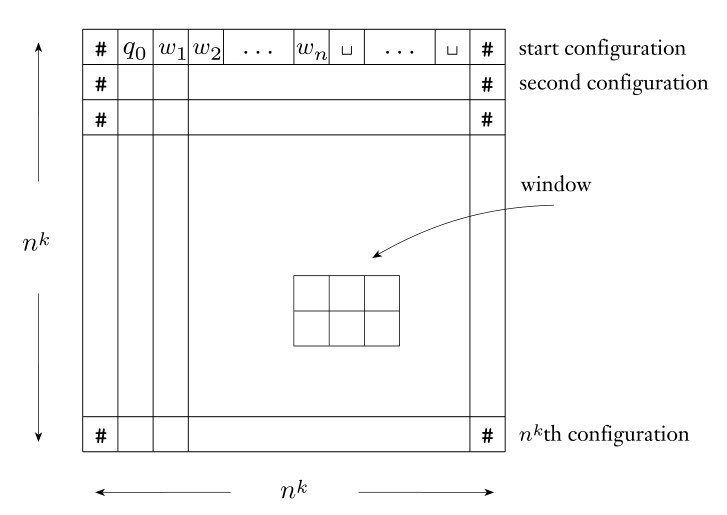
\includegraphics[scale=.5]{cooklevin.jpg}
		\caption{The tableux of configurations. We indexed from lower to upper, this is from the book.}
	\end{figure}
	The dimensions of this matrix is $t(n) \times  (t(n) + 3)$ (at most). The formula $\varphi$ will say "there exists such matrix of an accepting run". Let us construct it:\\
	Its variables are:
	\begin{align*}
		\forall i,j \text{ entry in the matrix, and } s\in S \text{ - assign a variable } x_{i,j,s}\text{ that describes }A^j_i = s
	\end{align*}
	$\varphi = \phi_{cell}\land \phi_{init} \land \phi_{acc} \land \phi$ With:
	\begin{itemize}
		\item $\phi_{cell}$ says "a satisfying valuation describes an accepting run" (that is, no $\nu(x_{1,1,a}) = \nu(x_{1,1,b})$)
		\item $\phi_{init}$ says "an assignment to the first row complies with the initial configuration of $\Mm$ over $w$".
		\item $\phi_{acc}$ says "there is a row that describes an accepting configuration".
		\item $\phi_{move}$ says "ascending in the matrix complies with transition between subsequent configurations".
	\end{itemize}
So:
\begin{align*}
		&\phi_{cell} = \bigwedge_{i,j}\left[\overbrace{\left(\bigvee_{s\in S} x_{i,j,s}\right)}^{\text{Every cell contains a letter}}\land \overbrace{\left(\bigwedge_{s_1\neq s_2} \neg x_{i,j,s_1}\lor \neg x_{i,j,s_2}\right)}^\text{Only one letter}\right]\\
		&\varphi_{init} =\overbrace{ x_{1,1,\#}\land x_{2,1,q_0}\land x_{3,1,w_1}\land\ldots x_{n+2,n,w_n}\land x_{n+3,1,\blank},\ldots\land x_{t(n) + 3, 1, \#}}^{\text{The first row is the initial configuratoin}}\\
		& \varphi_{acc} =\overbrace{ \bigvee_{j\in [t(n)]}\left[\bigvee_{2\leq i\leq t(n) + 2} x_{i,j,q_{acc}}\right]}^{\text{In some row there is $q_{acc}$}}\\
\end{align*}
For $\phi_{move}$ - it is sufficient to check submatrices of size $3\times 2$ (since legal transitions are very local). That is - there is a set $W$ of finite cardinality  of legal "windows" (submatrices) of size $3\times 2$. $\phi_{move}$ will say "all windows of size $3\times 2$ are from $W$":
\[
\phi_{move} = \bigwedge_{\underset{i\leq t(n) + 1}{j\leq t(n) - 1}}
\left[\bigvee_{(s_1,s_2,s_3,s_4,s_5,s_6)\in W}\overbrace{x_{i,j,s_1} \land x_{i+1,j, s_2}\land x_{i+2, j ,s_2}\land x_{i, j+1, s_4}\land x_{i+1, j+1, s_5}\land x_{i+2, j+1, s_6}}^{\text{the window is legal}} \right]
\]
We now define $W$ (and that it is of polynomial size in $n$). For any transition $\delta(q_1,a)\ni \tbk{q_2, b,R}$ (and of course similarly for $L$), add windows of the following types:\\
\begin{figure}[H]
	\centering
	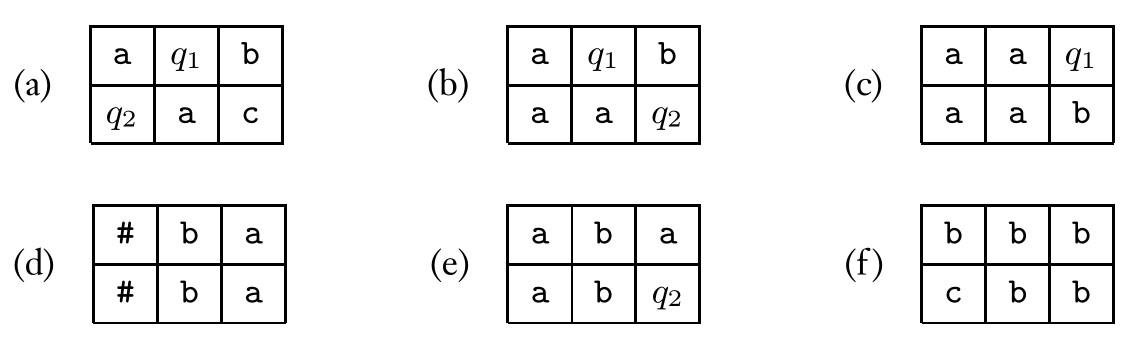
\includegraphics[scale=0.5]{cooklevinwindows.jpg}
	\caption{Examples of legal windows}
\end{figure}
And in sequential notation (for example) - $(q_1, a, c, b, q_2, b)$. So for any transition there is a finite number of valid windows. In fact - this is independent of $|w|$ - so we're all good.\\
We show that $\varphi$ is satisfyable iff there is an accepting run of $\Mm$ over $w$: Assume $f$ is a truthful valuation of $\phi$, then $f$ describes a matrix of size $(t(n) +3 )\times t(n)$. Since $\phi_{init}$ is satisfied - the first row describes the initial configuration of $\Mm$ on $w$. Since $\phi_{move}$ is satisfied - the $j+1$'s row is a subsequent configuration of the $j$'s row. Since $\phi_{acc}$ is satisfied - at some point, we reach an accepting configuration. Therefore - there is an accepting run of $\Mm$ on $w$.\\
Conversely - if there exists an accepting run of $\Mm$ over $w$, there is a matrix with the sequence of configuration describing a satisfying valuation of $\phi$.\\

All constructions are polynomial in $t(n)$, hence polynomial in $n$ - so the reduction is polynomial.\\

$\phi$ is in $CNF$ form, but not $3CNF$. We will show in the exercise that we can reform a formula in $CNF$ to a formula in $3CNF$ in polynomial time.
\end{proof}
\section{More examples}
As we defined $\NP$ hardness and $\NP$ completeness, there are symmetric definitions for $\coNP$ (as well as for any complexity class). We see some examples:
\begin{example}
	Define $VAL = \cbk{\tbk{\phi}\mid \text{All valuations satisfy $\phi$}}$. That is, for any $\nu:X\to \{T,F\}$ we have $\nu \vDash \phi$, iff there is no $\nu$ with $\nu \vDash \neg \varphi$ iff $\phi\notin SAT$. So $VAL\in \coNP$
\end{example}
\begin{blueBox}
	\begin{thm}
		$\Ll$ is $\coNP$-complete $\iff$ $\Ll^c$ is $\NP$-complete.
	\end{thm}
\end{blueBox}
\begin{proof}
	By definition, for any $\Ll'\in \coNP$ we have $\Ll'^c\in \NP$. Therefore there is a reduction $\Ll'^c\leq_p \Ll^c$ since $\Ll^c$ is $\NP$-hard. The same reduction implies $\Ll'\leq_p \Ll$, hence $\Ll$ is $\coNP$ hard.
\end{proof}
\subsection*{Another reduction $3SAT\leq_p CLIQUE$}
Given $\phi = {\displaystyle \bigwedge_{i\leq j\leq m}}\left(\ell^1_j \lor \ell^2_j \lor \ell^3_j\right)$, we would like to define an undirected graph $G$ and a number $k$ such that $K_k\subset G$ iff $\phi$ is satisfyable. Consider the clause $C_j = x_1\lor \neg x_2 \lor x_3$. There are $2^3-1$ satisfying valuations\footnote{Consider the equivalent disjunctive form of the clause}. We will consider these valuations as \textbf{restrictions}. Denote $F_j = \{\nu^l_j\}_{l\in [7]}$ the satisfying valuations of $C_j$ (over its three variables). Define $V(G) = {\displaystyle \bigcup_{j\in [m]} F_j}$.\\
\textbf{I can't find the example in my photos - If anyone could send it to me, that'd be great }\\
And let $E(G)$ be the set of edges with no "contradiction", that is $\{\nu^{l_1}_j,\nu^{l_2}_t\}\in E(G)$ agree on their common variables (and of course no loops). We claim $K_m\subset G$ iff there is a satisfying valuation.\\
Note that this construction is polynomial in $|\phi|$ - since there are at most $8\cdot m$ valuations to check (to defnie nodes), and the edges need at most $O(3\cdot m^2)$ things to check.
\begin{remark}
	This construction is exponential in $3$ - that is, for a fixed $k$, this will work for any $k-CNF$ class of formulas.
\end{remark}
\chapter{Space Complexity}
\section{Introduction}
\begin{yellowBox}
	\begin{defn}[Space Complexity]
		We say that a (single strip) TM $\Mm$ works in \textbf{Space Complexity} $S:\NN\to \NN$ if for any input $w$, $\Mm$ uses at most $S(|w|)$ cells of the strip.
	\end{defn}
\end{yellowBox}
As in time complexity - there are space complexity classes.
\begin{yellowBox}
	\begin{defn}
		Given $S:\NN\to \NN$, we define $$\SPACE(S(n)) = \tbk{\Ll\mid \Ll\text{ is decided by a TM with space compexity } O(S(n))}$$
	\end{defn}
\end{yellowBox}
\begin{blueBox}
	\begin{thm}
		$TIME(f(n))\subset \SPACE(f(n))$
	\end{thm}
\end{blueBox}
\begin{proof}
	If a TM works in time $f(n)$, it can reach with its head only to $f(n)$ cells.
\end{proof}
\begin{blueBox}
	\begin{thm}
		$\SPACE(f(n))\subset \TIME(2^{O(f(n))})$
	\end{thm}
\end{blueBox}
\begin{proof}
	We compute how many configurations exists to a TM $\Mm$ with space complexity $S(n)$: $|Q|\cdot S(n) \cdot |\Gamma|^{S(n)} = c_1 \cdot S(n) \cdot c_2^{S(n)} = 2^{O(S(n))}$.\\
	Since $\Mm$ decides a language and is deterministic, it does not repeat the same configuration twice. Therefore - it halts within $2^{O(S(n))}$ steps.
\end{proof}
\section{Space Complexity Classes}
\begin{yellowBox}
	\begin{defn}
		We define, similarly to time complexity classes:
		\begin{itemize}
			\item $\NSPACE(S(n)) = \cbk{\Ll\mid \text{$\Ll$ i decided by a nondeterministic TM with $O(S(n)$ space)}}$
			\item $\PSPACE = {\displaystyle \bigcup_{k\in \NN}\SPACE(n^k)}$
			\item $\NPSPACE = {\displaystyle \bigcup_{k\in \NN}\NSPACE(n^k)}$
		\end{itemize}
	\end{defn}
\end{yellowBox}
\begin{remark}
	By the previous theorems, we know:
	\[PTIMES\subset \PSPACE\qquad \PSPACE\subset EXPTIME\]
\end{remark}
\begin{example}
	$SAT\in \PSPACE$. The idea is to check all valuations of a given formula (by using the same space) one after the other (time-wise). Let $\nu_1\ldots \nu_{2^n}$ an ordering of the valuations (of $\phi$ with $n$ variables), such that given $\nu_i$, we can find $\nu_{i+1}$ with linear space - or return $\perp$ if we are in the last valuations (eg - lexicographic order). $\Mm$ operates the following way: One strip will hold $\nu_1$, the other the value $\nu(\varphi)$. While the first strip does not say $\perp$, $\Mm$ computes $\nu_i(\varphi)$. If $T$ -halt and accept. Otherwise - update in the first strip to the valuation $\nu_{i+1}$. When the first strip contains $\perp$ - reject.\\
	
	Note that the first strip requires $O(n)$ cells (and the space required for an update). The second strip needs $O(|\phi|)$ cells for computing $\nu(\phi)$.
	\end{example}
This can easily be extended for any language in $\NP$.
\begin{blueBox}
\begin{thm}
	$\NP\subset \PSPACE$
\end{thm}
\end{blueBox}
\begin{proof}
	Let $\Ll\in \NP$, ad let $\Vv$ be a polynomial verifier of $\Ll$, with $f:\NN\to \NN$ bounding  $\Vv$'s runtime. Let $c_1\ldots c_{|\Sigma|^{f(|w|)}}$ the lexicographic ordering of $\Sigma^{\leq f(|w|)}$. A TM that decides $\Ll$ in polyspace would go over all $c_i$ (the "witnesses") and simulate $\Vv$ to check them. The details can be completed as in the previous example.
\end{proof}
\begin{example}
	Denote $EMPTY_{NFA} = \cbk{\tbk{\Aa}\mid \Ll(\Aa) = \emptyset}$ and $ALL_{NFA} = \cbk{\tbk{\Aa}\mid \Ll(\Aa) = \Sigma^*}$ and consider their complements $\overline{EMPTY_{NFA}}, \overline{ALL_{NFA}}$. It is clear that $\overline{EMPTY_{NFA}}\in \NP$ - by the witness in the form of a word (of length corresponding to a simple path over $\Aa$'s graph, therefore polynomial in $\tbk{\Aa}$). We need to show that it can be verified in polytime (since $\Aa$ is nondeterministic it is not trivial). Consider the automaton $\Aa_w$  with $\Ll(\Aa_w) = \{w\}$. Then the product automaton $\Aa\times \Aa_w$\footnote{A variation of this} has the language $\Ll(\Aa)\cap \Ll(\Aa_w)$. So $w\in \Ll(\Aa)$ iff $\Ll(\Aa\times \Aa_w)\neq \emptyset$. Checking this is in fact checking if an accepting state is reachable from some initial state. In Algorithms course we saw that this is polynomial in the graph's size.\\
	
	For $\overline{ALL_{NFA}}$, how would we go about that? For $\overline{ALL_{DFA}}$ this is easy (since the complement automaton would have empty language). It is not clear that $\overline{ALL_{NFA}}\in \NP$. We will construct NFA $\Aa$ with $\Ll(\Aa)\neq \Sigma^*$, but the shortest word $\Aa$ rejects is exponential in $|\Aa|$:\\
	Let $i\geq 1$, consider the first $i$ prime numbers $p_1\ldots p_i$, and consider the language: $$\Ll_i = \cbk{w\mid |w| \text{ is not divisible by one of $p_1 \ldots p_i$}}$$
	Denote $\Aa_{p_j}$ the automaton with a cycle of size $p_j$ and the first state rejects. Then $\Aa_i = {\displaystyle \bigsqcup_{j\in [i]} A_{p_j}}$, and since $|p_j| = O(j\log j)$, $|\Aa_i|$ is polynomial in $i$. Consider $w^* = a^{\prod_{j\in i}p_j}$, then $w^*\notin \Ll_i$, but $|w^*| \geq 2^i= \exp(i)$. Then there is a word which is not in $\Ll_i = \Ll(\Aa_i)$. We need to show that $a^y$ with $y<\prod_{j\in i}p_j$ is accepted. This is because when we decompose $y$ into prime components, there must appear a component which is not in $\{p_j\}_{j\in [i]}$.
\end{example}
\begin{claim}
	$\overline{ALL_{NFA}}\in \NPSPACE$.
\end{claim}
\begin{proof}
	Given $\Aa$ NFA, the following are equivalent:
	\begin{enumerate}
		\item $\Ll(\Aa)\neq \Sigma^*$
		\item $\Ll(\overline{\Dd}) \neq \emptyset$\footnote{The accepting states of $\overline{\Dd}$ are exactly $S\subset Q$ such that $S\cap F = \emptyset$} with $\Dd$ the $DFA$ generated by the subset construction over $\Aa$.
		\item There exists an increasing sequence of states $\{Q_i\}_{i=0}^k$ with $k\leq 2^{|Q|}$ such that $Q_0$ is the set of initial states of $\Aa$, and for all $i$, $Q_{i+1} = \delta(Q_i, \sigma_i)$ for some $\sigma$, and $Q_k\cap F = \emptyset$ (that is, this is a sequence corresponding to an accepting run of some word in $\overline{\Dd}$).
	\end{enumerate}
	$(1\iff 2)$ Since $\Ll(\overline{\Dd}) = \Sigma^\setminus \Ll(\Aa)$, this is immediate.\\
	$(2\iff 3)$ $\Ll(\overline{\Dd})\neq \emptyset \iff$ there is a word with length $\leq 2^{|Q|}$ (number of states of $\overline{\Dd}$) that is accepted (because there is a word that's accepted over a simple path) $\iff$ there exists the required sequence.\\
	
	Then define an NTM operating in polyspace $\Mm$ and decides $\overline{ALL_{NFA}}$: On the strip we will hold a counter (until $2^{|Q|}$, requires $O(|Q|)$ space!) and the encoding of the current state $S = Q_{i}$ (an instance of a subset of $Q$, lets say represented by a subset of $[n]$ - still polyspace in $|Q|$)
	\begin{enumerate}
		\item Write $Q_0$ on the strip (where we keep states)
		\item writes $i=0$ (where we keep counter)
		\item While $i\leq 2^{|Q|}$:
		\begin{enumerate}[3.1]
			\item If $Q_i \cap F = \emptyset$ - halt and accept
			\item Otherwise - \textbf{guess} a letter $\sigma\in \Sigma$ and updates the strips: $Q_i$ is substituted with $\delta(Q_i, \sigma)$ and $i++$.
		\end{enumerate}
	\item Halt and reject
	\end{enumerate}
\end{proof}
\begin{blueBox}
	\begin{thm}[Savitch Theorem]
		For any space complexity $S$ with $S(n) \geq n$, \[\NSPACE(S(n)) \subset \SPACE(S^2(n))\]
	\end{thm}
\end{blueBox}
\begin{proof}
	Let $\Nn\in \NSPACE(S(n))$. Preliminaries: 
	\begin{itemize}
		\item For any $w$, $\Nn$ has a unique initial configuration $C_{init}^w$.
		\item $\Nn$ has a unique accepting configuration (say, when $\Mm$ arrives at an accepting configuration - it cleans the strip and goes back to the beginning of the strip), denoted $C_{acc}$.
		\item Let $d$ be such that $\Nn$ has at most $2^{d\cdot S(n)}$ different configurations during a run over a word of length $n$.
	\end{itemize} 
We build a deterministic procedure\footnote{A part of a TM, we will iteratively run this procedure} $\Mm = reach(C_1, C_2, t)$ that decides if the configuration $C_2$ is reachable from $C_1$ within $t$ steps. Its space complexity would be $O(\log(t) + S(n))\cdot \log(t)$. Then given $w$, an NTM $\Mm'$ would check $reach(C_{init}^w, C_{acc}, 2^{d\cdot S(|w|)})$. Note that indeed $\Mm$ accepts $w$ iff $reach(C_{init}^w, C_{acc}, 2^{d\cdot S(|w|)})$, and that the space complexity would be $O(S^2(n))$.\\

The procedure:
\begin{enumerate}
	\item If $C_1 = C_2$ or $C_2$ is subsequent of $C_1$ - accept.
	\item Otherwise - Iterate over all configurations $C$ that use $S(|w|)$ cells. For each of them:
	\begin{enumerate}[2.1]
		\item Check if $reach(C_1, C, \lceil\frac{t}{2}\rceil)$
		\item Check if $reach(C, C_2, \lfloor\frac{t}{2}\rfloor)$
		\item If both accepted - accept.
	\end{enumerate}
\item Reject
\end{enumerate}
Correctness is obvious. The hard part is checking the space complexity. The recursion's depth is $log(t)$. The recursion "saves" only one branch of the recursion tree in any given moment. Hence we save only the path from the root to the current node, and information related to iterating over all configurations. That is - to save a single node, we need:
\[2\cdot S(n) + \log(t)\]
space to save any node (two configurations $S(n)$ and current path length $\log(t)$), information to iterate over configurations is $S(n)$, so total space complexity $O(S(n) + \log(t))\cdot \log(t)$.\\
How does $reach$ "knows" $S(n)$? If $S(n)$ is known - everything's fine. If $S(n)$ is unknown, build the same TM with a twist. Note that $reach$ can be used to check if there exists a reachable configuration that uses $i$ cells: Iterate over all configurations that uses $i$ cells, and for each such $C$, check $reach(C_{init}^w, C, 2^{di})$ (assuming $S(n) = i$). We build an outer loop to deterministically decide if $\Mm$ accepts $w$:
\begin{enumerate}
	\item For $i\in \NN$:
	\begin{enumerate}
		\item Check if there is a reachable configuration that uses $i$ cells? If not - reject
		\item If there is - run the previously built $\Mm$ with $S(n) = i$. If accepted - accept. Otherwise, $i++$.
	\end{enumerate}
\end{enumerate}
\end{proof}

\begin{cor}
	$$\NPSPACE = \PSPACE = \coNPSPACE = \coPSPACE$$
\end{cor}

\section{Space-Hardness and Space-Completeness}
\begin{yellowBox}
	\begin{defn}[$\PSPACE$-hard]
		We say that $\Ll$ is \textbf{$\PSPACE$-hard} if for any $\Ll'\in \PSPACE$, $\Ll'\leq_p \Ll$. 
	\end{defn}
\begin{remark}
	The same notation of $\leq_p$ as in time complexity.
\end{remark}
	\begin{defn}[$\PSPACE$ - complete]
		We say that $\Ll$ is \textbf{$\PSPACE$-complete} if $\Ll\in \PSPACE$ and is $\PSPACE$-hard.
	\end{defn}
\end{yellowBox}
We will see a $\PSPACE$-complete language. For this we need a new definition regarding boolean formulas:
\begin{yellowBox}
	\begin{defn}
		We say a formula $\phi$ is \textbf{Fully Quantified} if any variable $x\in \phi$ is connected to a quantifier $\exists, \forall$
	\end{defn}
\end{yellowBox}
\begin{example}
	Define $TQBF = \cbk{\tbk{\phi}\mid \phi\text{ is a True fully quantifid formula}}$. That is, $\phi\in TQBF$ is a totally quantified tautology.
	\begin{claim}
		$TQBF\in \PSPACE$
	\end{claim}
\begin{proof}
	Define $\Mm$ to operate recursively over $\phi$:\begin{enumerate}
		\item (Base Case) If $\phi$ is without quantifier, then $\Mm$ valuates $\phi$ and accepts if True. Otherwise - reject.
		\item If $\phi = (\exists x) \psi$, then run $\Mm(\psi)$ recursively twice: once with $x = 0$ and once with $x=1$. Accept if one of them accepts - accept. Otherwise reject.
		\item If $\phi = \forall x \psi$ then run $\Mm(\psi)$ recursively with $x=0$ and with $x=1$. Accept if both accepted. Otherwise reject.
	\end{enumerate}
This obviously decides $TQBF$. Note that the depth of enery branch in the recursion tree is bounded by number of variables of $\phi$ $\leq |\phi|$, and for any variable we run at most twice. In every stage we remember which variables were substituted and what's left to check - $O(|\phi|)$ space. Finally, in the base case we valuate $\phi$ which takes $O(|\phi|)$ space - all in all, the space complexity is $O(|\phi|^2)$ - as required.
\end{proof}
We would like not wo show it is complete in $\PSPACE$. How do we encode configurations using boolean formulas?\\
Let $\Mm$ be a TM and assume $\Mm$ uses $S$ strip cells. Encode the following way:
\begin{enumerate}
	\item For $i\in [S]$ define a variable $x_{ia}$ which encodes "$a$" is written in cell $i$".
	\item For $i\in [S]$ define a variable $y_i$ which encodes "The reading head is over cell $i$"
	\item For any $q\in Q$ define a variable $z_q$ which encodes "The machine $\Mm$ is in state $q$".
\end{enumerate}
\begin{blueBox}
	\begin{thm}
		Let $\Mm$ be a TM. Then:
		\begin{enumerate}
			\item There exists a formula $\phi_{valid}(C)$ which is True iff $C$ is a valid encoding of a configuration of $\Mm$.
			\item There exists a formula $\phi(C_1,C_2)$ which is True iff $C_2$ is subsequent of $C_1$.
		\end{enumerate}
	In addition - both formulas are computable in polyspace in $S$.
	\end{thm}
\end{blueBox}
\begin{proof}
	Define:
	\[
	\phi_{valid}(C) = \bigwedge_{i\in [S]}\bigvee_{a\in \Gamma}\left(x_{ia}\land \bigwedge_{b\in \Gamma\setminus\{a\}}\neg x_{ib}\right)\land\bigvee_{i\in [S]}\left(y_i\land \bigwedge_{j\in [S]\setminus \{i\}}\neg y_j\right)\land\bigvee_{q\in Q}\left(z_q\land \bigwedge_{q'\in Q\setminus\{q\}}z_{q'}\right)
	\]
	Note that $|\phi_{valid}(C) = O(S^2)$. Now define for any $i\in [S], a\in \Gamma, q\in Q$, if $\delta(q,a) = (r,b,R)$ then define:
	\[
	\psi_{iaq}(C_1,C_2) = (x^1_{ia}\land y^1_i\land z^1_q)\Rightarrow (x^2_{i,b}\land y^2_{i+1}\land z_r\bigwedge_{j\in [S]\setminus \{i\}}\bigwedge_{d\in \Gamma}(x^1_{jd}\iff x^2_{jd}))
	\]
	And of course, symmetrically define for transition to $L$, and for exceptions (e.g - when we are in cell $1$ and move to the left).
	Convince yourself that this actually encodes the transition. Now define:
	\[
	\phi(C_1, C_2) = \phi_{valid}(C_1)\land \phi_{valid}(C_2) \land \bigwedge_{i\in [S]}\bigwedge_{a\in \Gamma}\bigwedge_{q\in Q}\psi_{iaq}(C_1,C_2)
	\]
	Once again - the length of $\psi(C_1, C_2) = O(S^2)$
\end{proof}
\begin{claim}
	$TQBF$ is $\PSPACE$-hard.
\end{claim}
\begin{proof}
	Let $\Ll\in \PSPACE$ be a language. We would like to build a function $f:w\mapsto\phi_{w}$ such that $w\in \Ll\iff \phi_w\in TQBF$. Let $\Mm$ be a TM that decides $\Ll$ is polyspace. \\
	Define a formula that says "$C_2$ is reachable from $C_1$ within $k$ steps": 
	\[
	\phi_k(C_1,C_2) = \exists C_m\forall C_3,C_4\left[(C_3 = C_1)\land (C_4 = C_m)\lor (C_3=C_m)\land(C_4 = C_2)\right]\Rightarrow \phi_{k/2}(C_3,C_4)
	\]
	Any recursive call is polynomial and there is only one branch - so no exponential number of leaves. This formula is built in polyspace in $w$.
\end{proof}
\end{example}
\begin{example}
	Consider the language $\overline{ALL_{NFA}}$. We've shown that $\overline{ALL_{NFA}}\in \NPSPACE$. By Savitch - $\overline{ALL_{NFA}}, ALL_{NFA}\in \PSPACE$. We will see that $\overline{ALL_{NFA}}$ is $\PSPACE$-hard.
\end{example}
\section{Sublinear Space Complexity}
\begin{yellowBox}
	\begin{defn}
		Define $$LOGSPACE = \SPACE(\log(n)), NLOGSPACE =\NSPACE(\log(n))$$ denoted $L,NL$ respectively.
	\end{defn}
\begin{remark}
	Since the input itself takes $|w|$ space, we change the computational model a little: We require two strips, and that the work strip would be of logarithmic space.
\end{remark}
\end{yellowBox}
\begin{example}
	Let $EQ = \{0^k1^k\mid k\in NN_0\}$. We saw that $EQ\in \P$, but the algorithm wrote on all of the cells, thus $EQ\in \SPACE(n)$. We define a TM $\Mm$ that decides $EQ$ in $LOGSPACE$. The machine maintains two counters $C_0, C_1$ in binary, and counts. each counter takes $O(\log(n))$ cells. Then compares them.
\end{example}
\begin{example}
	Recall $PATH = \cbk{\tbk{G,s,t}\mid G\text{ is a directed graph and there is a path }s\to t}\in \P$. We show $PATH\in NLOGSPACE$ by guessing a path. We only need to "remember" on which node we stand in any given moment moment. We also maintain a counter $i$ until $|V|$ (once again, in binary). $\Mm$ operates the following way:
	\begin{enumerate}
		\item Write on the strip $s_0 = s, i=0$.
		\item While $i\leq |V|$, if $s_i = t$ then halt and accept. Otherwise - guess a neighbor $s_i\to s_{i+1}$, and $i++$.  
		\item Halt and reject.
	\end{enumerate}
Correctness is clear: There is a path $s\to t$ iff there is a simple path $s\to t$ iff $\Mm$ might guess this path iff $\Mm$ accepts.\\

Is $PATH\in LOGSPACE$? By Savitch. $\NSPACE(s(n))\subset \SPACE(s^2(n))$, but this does not imply $NLOGSPACE\subset LOGSPACE$
\end{example}
\subsection*{Completeness and Hardness}
The definitions are the same - with a twist: Polynomial reductions are not good enough\footnote{We will see that $NL\subset \PTIME$} - so we need a new notion of reduction:
\begin{yellowBox}
	\begin{defn}[Logspace Reduction]
		A function $f:\Sigma^*\to \Sigma^*$ is a \textbf{Logspace Reduction} if there exists a \textbf{Logspace transducer} $\Mm$. That is, $f$ is computable by $\Mm$ which operates with $3$ strips (input - RO, work - RW, and output - WO): The work strip is with $O(\log(|w|)$ cells, and $\Mm$ writes $f(w)$ on the output strip.
	\end{defn}
\begin{remark}
	If $f$ is such that $w\in \Aa \iff f(w)\in \Bb$, we write $\Aa\leq_L \Bb$.
\end{remark}
\end{yellowBox}
\begin{example}
	Consider a digraph with two types of nodes. An initial node $s$ holds a token. The first type node ("first player") does not want the token to reach $t$, and the second type node ("second player") wants the token to reach $t$. This problem is in $\P$ and in fact is $\P$-complete.
\end{example}
\begin{blueBox}
	\begin{thm}
		$PATH$ is $NL$-complete.
	\end{thm}
\end{blueBox}
\begin{proof}
	It is left to show that for any $\Ll\in NL$, $\Ll\leq_L PATH$. The idea: let $\Mm$ be a logspace decider of $\Ll$. The graph $G$ would be the configurations graph, $s=  C^w_{init}$ and $t = C_{acc}$ the accepting configuration (as always, assume uniqueness). $G$'s nodes would be all configurations, and edges iff subsequent configurations.\\
	Any configuration is described by an element of $\Gamma^i (\Gamma\times Q)\Gamma^{s(n) - i+1}\# (0+1)^{\log(n)}$, which requires $2\log(n) + 1 = O(\log(n))$ space. The reduction go over all words over $\Gamma\cup (Q\times \Gamma)\cup \{\#,0,1\}$ and write those who describe a valid configuration. These are $V(G)$. For $E$, iterate over pairs of words and copy those who correspond to subsequent configurations. For $s,t$ - we just write them down, as we know their structure.
\end{proof}
\begin{remark}
	There were some results for which we demanded $s(n) \geq n$. This is because we bounded the number of configurations with $2^{ds(n)}$ for some $d$, and wanted to notice something exponential. Even when $s(n) = O(\log(n))$, there exists $d$ such that the number of configurations is bounded by $2^{d\cdot s(n)}$: In this case, the number of configurations is $|Q|\cdot |\Gamma|^{s(n)}\cdot s(n)\cdot n$ with the $n$ indicating the reading head's location in the input strip. When $s(n) = O(\log(n))$, the number of configurations is bounded by $k_1\cdot k_2^{d_1 \log(n)}(d_1\log(n))2^{\log(n)}\leq 2^{d\log(n)}$ for some $d$. Hence Savich holds even in logspace.
\end{remark}
\begin{blueBox}
	\begin{thm}
		$NL\subset \P$
	\end{thm}
\end{blueBox}
\begin{proof}
	Let $\Ll\in NL$. Reduce $\Ll\leq_L PATH$ (takes polytime since the number of configurations of $\Ll$ is polynomial). Afterwards run $DFS$ or $BFS$ (in polytime) and respond accordingly.
\end{proof}